
\section{Prepare data}
\label{sec:dataPrepare}
\subsection{Raw data}

Data should be prepared as the example in Figure~\ref{fig:dataMicroarray}.
First column should be feature ID (e.g. gene symbol) and the rest of the columns are samples.
Note that the first column can also be other feature type (i.e. probe id, entrez ID).
The first row is sample ID.
Valid data type includes continuous data and count data.

\begin{figure}[H]
\begin{center}
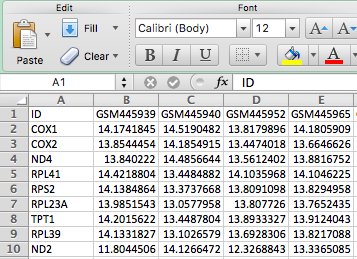
\includegraphics[scale=0.5]{./figure/dataPreparation/dataMicroarray}
\caption{A example input data format}
\label{fig:dataMicroarray}
\end{center}
\end{figure}

\subsection{Clinical data}

Clinical data should be prepared as the example in Figure~\ref{fig:clinical}.
First column should be sample ID and each row represents a sample.
The rest of the columns are clinical information.

\begin{figure}[H]
\begin{center}
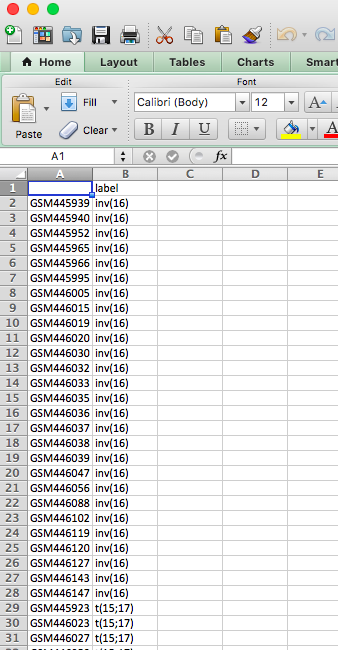
\includegraphics[scale=0.5]{./figure/dataPreparation/clinicalData}
\caption{A example clinical data format}
\label{fig:clinical}
\end{center}
\end{figure}

\subsection{Example data with the MetaOmics software}

\subsubsection{Leukemia datasets}

We collected three studies from NCBI GEO website.   
The original datasets are due by \cite{verhaak2009prediction}, \cite{balgobind2011evaluation} and \cite{kohlmann2008international}.	
This this example we  considered samples from acute myeloid leukemia (AML) with subtype 
	inv(16)(inversions in chromosome 16), 
	t(15;17)(translocations between chromosome 15 and 17), 
	t(8;21)(translocations between chromosome 8 and 21).
	These AML subtypes have been well-studied with different survival, 
	treatment response and prognosis outcomes.
	

			\begin{table}	
			\caption{Leukemia dataset information}						
			\centering
			\begin{tabular}{  c | c  c  c }
				 \hline
				 \hline
				Study Name &  Study 1 & Study 2 & Study 3 \\ 
				\hline
				Source &  Verhaak at el. & Balgobind at el. & Kohlmann at el. \\ 
				Number of genes  & 5,135 & 5,135 & 5,135 \\ 
				Number of patients   & 89 & 74 & 105 \\ 
				\hline
				 Platform & \multicolumn{3}{ c }{Affymetrix human genome u133 plus 2.0 array }\\ 
				 \hline
				 \hline
			\end{tabular}
			\label{tab:realDataLeukemia}
		\end{table}

\subsubsection{Prostate cancer datasets}
